\setlength{\resLen}{.13\columnwidth}
\begin{figure}[t]
	\addtolength{\tabcolsep}{-4pt}
	\begin{tabular}{ccccccc}
		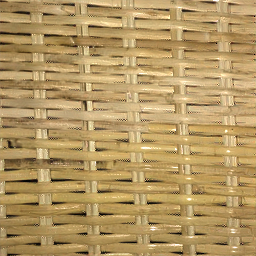
\includegraphics[width=\resLen]{others/matgan/04.jpg} &
		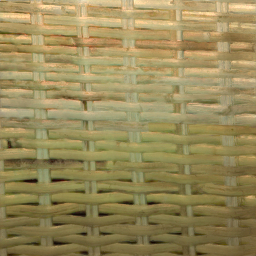
\includegraphics[width=\resLen]{others/matgan/05.jpg} &
		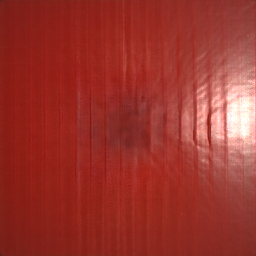
\includegraphics[width=\resLen]{others/matgan/08.jpg} &
		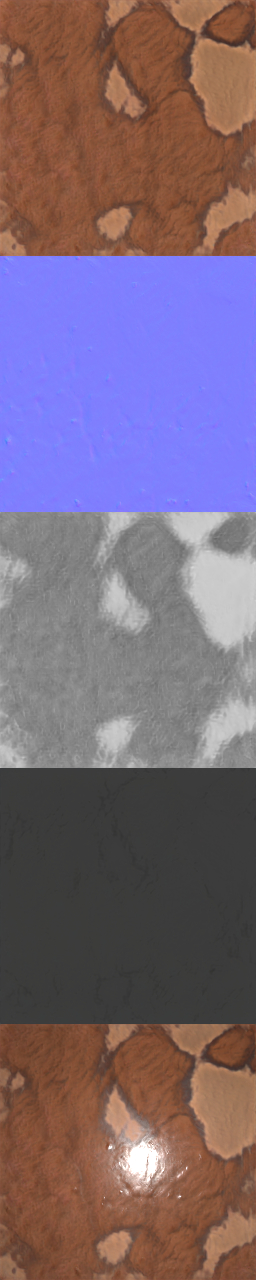
\includegraphics[width=\resLen]{others/matgan/10.jpg} &
		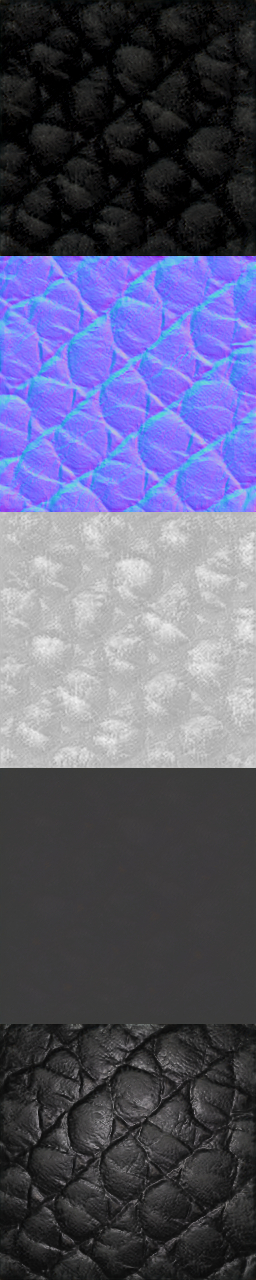
\includegraphics[width=\resLen]{others/matgan/11.jpg} &
		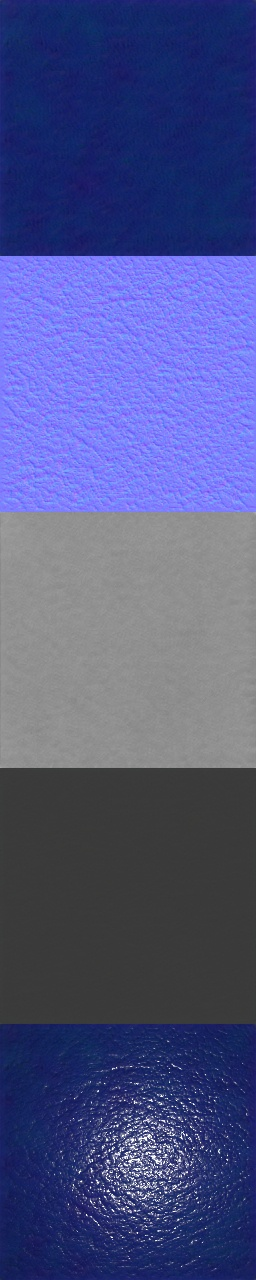
\includegraphics[width=\resLen]{others/matgan/12.jpg} &
		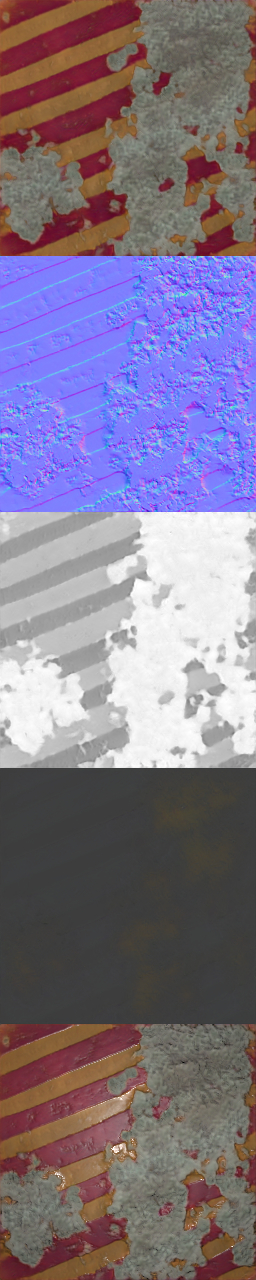
\includegraphics[width=\resLen]{others/matgan/19.jpg}
	\end{tabular}
	\caption{Seven materials generated by randomly sampling MaterialGAN. Top to bottom: diffuse albedo, normal, roughness, specular albedo and renderings under flash illumination. As can be seen, the material maps are high-quality with meaningful correlations both spatially and across materials parameters, and visually look like plausible real-world materials.
	}
	\label{fig:material_gan_samples}
\end{figure}